\documentclass[12pt, letter]{article}

\usepackage[margin=0.8in]{geometry}
\usepackage{amsmath}
\usepackage{tikz}
\usepackage{graphicx}
\graphicspath{ {./images/} }

\title{CS 381 - A4}
\author{Martin Mueller}
\date{Due: Friday, March $6^{th}$, 2020}

\begin{document}
	\maketitle
	\begin{enumerate}
		\item (10 points) Prove that the language  $\left\{ \left. 0^n1^m \; \right| \; n \ne m \right\}$ is not regular.
		\begin{center}
			Let's call the above language $L$. For the sake of obtaining a contradiction, assume $L$ is regular. Let $p$ be the pumping length given by the Pumping Lemma. Let $s = 0^{p}1^{p + p!}$. Since $|s| \ge p$, the Pumping Lemma says we can write $s = xyz$ where $|xy| \le p$, $|y| > 0$, and $xy^{i}z \in L$ for all $i \ge 0$. From this, we know that $y$ must be comprised of entirely zeros because $|xy| \le p$. We can now rewrite $s$ as $0^{p - q}0^{qi}1^{p + p!}$ for all $i \ge 0$. If we chose to pump up $s$ by setting $i = 1 + p!/q$ where $q$ is $|y|$, then we arrive at
			\begin{align*}
				s &= 0^{p - q}0^{q(1 + p!/q)}1^{p + p!} \\
				&= 0^{p - q + q + p!q/q}1^{p + p!} \\
				&= 0^{p + p!}1^{p + p!} \not\in L
			\end{align*}
			As we can see, pumping up the string $s$ yields a string that is no longer in the language. Therefore, $L$ is not a regular language by the pumping lemma because the string $xy^{i}z$ is not in $L$ for all possible values of $i$ greater than 0.
		\end{center}
		\pagebreak
%		\item (0 points) This problem is listed just for fun. Let $A$ be any language and define the set $A_{\frac{1}{3} - \frac{1}{3}} = \left\{ xz \mid \exists y, |x|=|y|=|z| \wedge xyz\in A \right\}$. Here, $A_{\frac{1}{3} - \frac{1}{3}}$ is roughly the set of all strings in $A$ with the middle thirds removed. \\
%		Show that, if $A$ is regular, then $A_{\frac{1}{3} - \frac{1}{3}}$ is not necessarily regular. \\
%		Do not use the Pumping Lemma. Hint: use closure operations. 

		\item (10 points) Convert the given machine into a corresponding regular expression. \\
		\includegraphics[scale=0.3]{convert-to-regex}
\begin{center}
	Constructed initial GNFA by adding a new start state with a $\lambda$ transition to the old start state, adding a new accept state that replaces all other accept states, adding $\lambda$ transitions from the old accept states to the new accept state, and adding $\emptyset$ transitions where needed.
\end{center}
\begin{center}
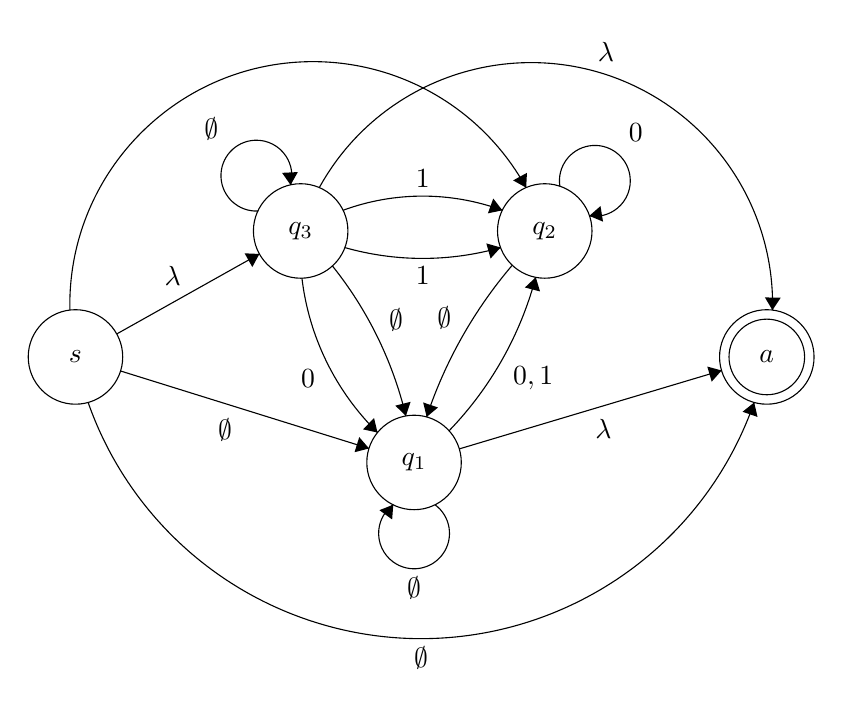
\begin{tikzpicture}[scale=0.2]
\tikzstyle{every node}+=[inner sep=0pt]
\draw [black] (14.8,-23.3) circle (3);
\draw (14.8,-23.3) node {$s$};
\draw [black] (29.1,-15.3) circle (3);
\draw (29.1,-15.3) node {$q_3$};
\draw [black] (44.6,-15.3) circle (3);
\draw (44.6,-15.3) node {$q_2$};
\draw [black] (36.3,-30) circle (3);
\draw (36.3,-30) node {$q_1$};
\draw [black] (58.7,-23.3) circle (3);
\draw (58.7,-23.3) node {$a$};
\draw [black] (58.7,-23.3) circle (2.4);
\draw [black] (17.42,-21.84) -- (26.48,-16.76);
\fill [black] (26.48,-16.76) -- (25.54,-16.72) -- (26.03,-17.59);
\draw (20.97,-18.8) node [above] {$\lambda$};
\draw [black] (57.899,-26.189) arc (-19.32901:-160.67099:22.412);
\fill [black] (57.9,-26.19) -- (57.16,-26.78) -- (58.11,-27.11);
\draw (36.75,-41.68) node [below] {$\emptyset$};
\draw [black] (14.445,-20.326) arc (-178.75637:-331.18941:15.444);
\fill [black] (43.42,-12.55) -- (43.47,-11.61) -- (42.59,-12.09);
\draw (24.76,-4.48) node [above] {${}$};
\draw [black] (30.283,-12.548) arc (151.13304:-1.38105:15.346);
\fill [black] (59.06,-20.33) -- (59.58,-19.54) -- (58.58,-19.52);
\draw (48.49,-4.58) node [above] {$\lambda$};
\draw [black] (26.393,-14.034) arc (272.65981:-15.34019:2.25);
\draw (23.42,-9.53) node [above] {$\emptyset$};
\fill [black] (28.46,-12.38) -- (28.92,-11.56) -- (27.92,-11.61);
\draw [black] (45.56,-12.47) arc (189:-99:2.25);
\draw (49.9,-9.05) node [right] {$0$};
\fill [black] (47.43,-14.34) -- (48.3,-14.71) -- (48.14,-13.72);
\draw [black] (37.623,-32.68) arc (54:-234:2.25);
\draw (36.3,-37.25) node [below] {$\emptyset$};
\fill [black] (34.98,-32.68) -- (34.1,-33.03) -- (34.91,-33.62);
\draw [black] (17.66,-24.19) -- (33.44,-29.11);
\fill [black] (33.44,-29.11) -- (32.82,-28.39) -- (32.52,-29.35);
\draw (24.3,-27.21) node [below] {$\emptyset$};
\draw [black] (39.17,-29.14) -- (55.83,-24.16);
\fill [black] (55.83,-24.16) -- (54.92,-23.91) -- (55.2,-24.87);
\draw (48.32,-27.2) node [below] {$\lambda$};
\draw [black] (33.983,-28.101) arc (-134.56275:-173.2464:16.483);
\fill [black] (33.98,-28.1) -- (33.76,-27.18) -- (33.06,-27.9);
\draw (30.04,-24.69) node [left] {$0$};
\draw [black] (31.115,-17.52) arc (38.69539:13.49546:24.316);
\fill [black] (35.78,-27.05) -- (36.08,-26.15) -- (35.11,-26.39);
\draw (34.68,-20.94) node [right] {$\emptyset$};
\draw [black] (37.097,-27.109) arc (161.60255:139.49706:28.853);
\fill [black] (37.1,-27.11) -- (37.82,-26.51) -- (36.88,-26.19);
\draw (38.69,-20.81) node [left] {$\emptyset$};
\draw [black] (44.026,-18.242) arc (-14.892:-44.00839:22.265);
\fill [black] (44.03,-18.24) -- (43.34,-18.89) -- (44.3,-19.14);
\draw (42.56,-24.68) node [right] {$0,1$};
\draw [black] (31.791,-13.986) arc (110.1747:69.8253:14.669);
\fill [black] (41.91,-13.99) -- (41.33,-13.24) -- (40.99,-14.18);
\draw (36.85,-12.59) node [above] {$1$};
\draw [black] (41.795,-16.355) arc (-74.14375:-105.85625:18.099);
\fill [black] (41.8,-16.35) -- (40.89,-16.09) -- (41.16,-17.05);
\draw (36.85,-17.54) node [below] {$1$};
\end{tikzpicture}
\end{center}
\pagebreak
\begin{center}
	Ripped state state $q_1$ and updated all transitions as needed.
\end{center}
\begin{center}
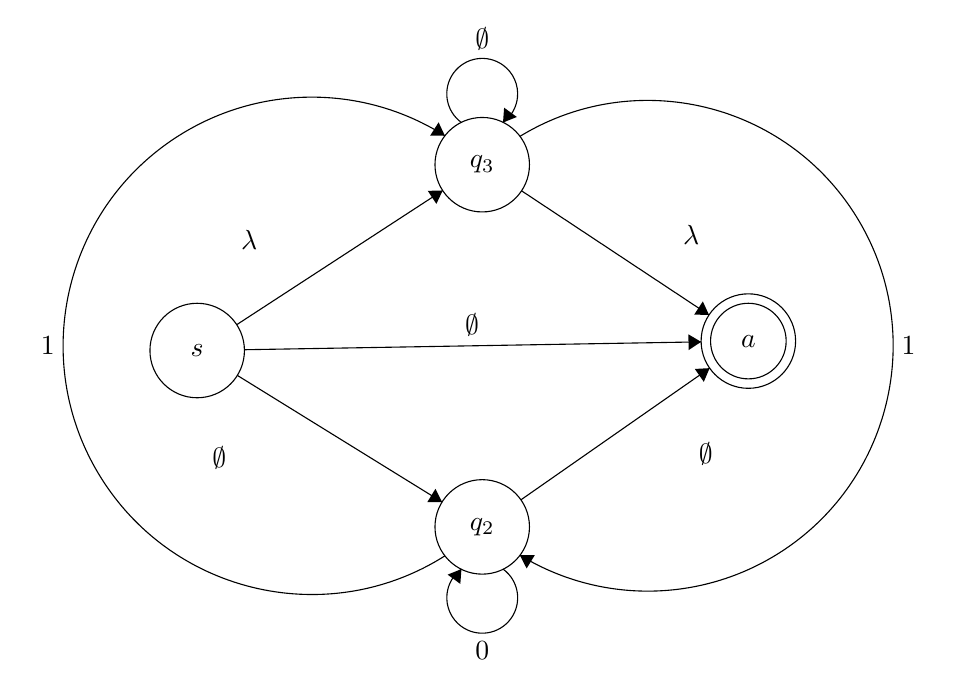
\begin{tikzpicture}[scale=0.2]
\tikzstyle{every node}+=[inner sep=0pt]
\draw [black] (56.6,-29.4) circle (3);
\draw (56.6,-29.4) node {$a$};
\draw [black] (56.6,-29.4) circle (2.4);
\draw [black] (21.6,-30) circle (3);
\draw (21.6,-30) node {$s$};
\draw [black] (39.7,-18.2) circle (3);
\draw (39.7,-18.2) node {$q_3$};
\draw [black] (39.7,-41.2) circle (3);
\draw (39.7,-41.2) node {$q_2$};
\draw [black] (24.11,-28.36) -- (37.19,-19.84);
\fill [black] (37.19,-19.84) -- (36.24,-19.86) -- (36.79,-20.69);
\draw (24.9,-23.6) node [above] {$\lambda$};
\draw [black] (24.6,-29.95) -- (53.6,-29.45);
\fill [black] (53.6,-29.45) -- (52.79,-28.97) -- (52.81,-29.97);
\draw (39.06,-29.1) node [above] {$\emptyset$};
\draw [black] (24.15,-31.58) -- (37.15,-39.62);
\fill [black] (37.15,-39.62) -- (36.73,-38.78) -- (36.21,-39.63);
\draw (23,-36.1) node [below] {$\emptyset$};
\draw [black] (42.2,-19.86) -- (54.1,-27.74);
\fill [black] (54.1,-27.74) -- (53.71,-26.88) -- (53.16,-27.72);
\draw (52.97,-23.3) node [above] {$\lambda$};
\draw [black] (42.16,-39.48) -- (54.14,-31.12);
\fill [black] (54.14,-31.12) -- (53.2,-31.17) -- (53.77,-31.99);
\draw (53.9,-35.8) node [below] {$\emptyset$};
\draw [black] (38.377,-15.52) arc (234:-54:2.25);
\draw (39.7,-10.95) node [above] {$\emptyset$};
\fill [black] (41.02,-15.52) -- (41.9,-15.17) -- (41.09,-14.58);
\draw [black] (41.023,-43.88) arc (54:-234:2.25);
\draw (39.7,-48.45) node [below] {$0$};
\fill [black] (38.38,-43.88) -- (37.5,-44.23) -- (38.31,-44.82);
\draw [black] (37.334,-43.037) arc (-57.62159:-302.37841:15.792);
\fill [black] (37.33,-16.36) -- (36.93,-15.51) -- (36.39,-16.36);
\draw (12.59,-29.7) node [left] {$1$};
\draw [black] (42.095,-16.401) arc (121.40162:-121.40162:15.581);
\fill [black] (42.09,-43) -- (42.52,-43.84) -- (43.04,-42.99);
\draw (66.29,-29.7) node [right] {$1$};
\end{tikzpicture}
\end{center}
\begin{center}
	Ripped state state $q_2$ and updated all transitions as needed.
\end{center}
\begin{center}
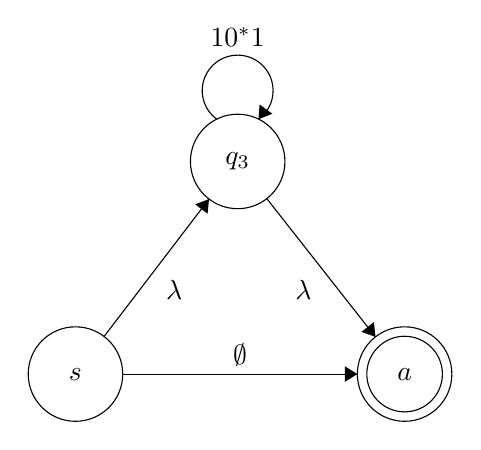
\begin{tikzpicture}[scale=0.2]
\tikzstyle{every node}+=[inner sep=0pt]
\draw [black] (29.1,-33.4) circle (3);
\draw (29.1,-33.4) node {$s$};
\draw [black] (39.4,-19.9) circle (3);
\draw (39.4,-19.9) node {$q_{3}$};
\draw [black] (50,-33.4) circle (3);
\draw (50,-33.4) node {$a$};
\draw [black] (50,-33.4) circle (2.4);
\draw [black] (30.92,-31.01) -- (37.58,-22.29);
\fill [black] (37.58,-22.29) -- (36.7,-22.62) -- (37.49,-23.22);
\draw (34.82,-28.05) node [right] {$\lambda$};
\draw [black] (38.077,-17.22) arc (234:-54:2.25);
\draw (39.4,-12.65) node [above] {$10^{*}1$};
\fill [black] (40.72,-17.22) -- (41.6,-16.87) -- (40.79,-16.28);
\draw [black] (41.25,-22.26) -- (48.15,-31.04);
\fill [black] (48.15,-31.04) -- (48.05,-30.1) -- (47.26,-30.72);
\draw (44.13,-28.07) node [left] {$\lambda$};
\draw [black] (32.1,-33.4) -- (47,-33.4);
\fill [black] (47,-33.4) -- (46.2,-32.9) -- (46.2,-33.9);
\draw (39.55,-32.9) node [above] {$\emptyset$};
\end{tikzpicture}
\end{center}
\begin{center}
	Ripped state state $q_3$ and updated all transitions as needed.
\end{center}
\begin{center}
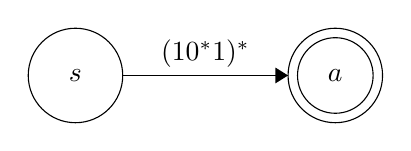
\begin{tikzpicture}[scale=0.2]
\tikzstyle{every node}+=[inner sep=0pt]
\draw [black] (29.1,-33.4) circle (3);
\draw (29.1,-33.4) node {$s$};
\draw [black] (45.6,-33.4) circle (3);
\draw (45.6,-33.4) node {$a$};
\draw [black] (45.6,-33.4) circle (2.4);
\draw [black] (32.1,-33.4) -- (42.6,-33.4);
\fill [black] (42.6,-33.4) -- (41.8,-32.9) -- (41.8,-33.9);
\draw (37.35,-32.9) node [above] {$(10^*1)^*$};
\end{tikzpicture}
\end{center}
	\end{enumerate}
\end{document}